\section{Câu 6}
    Thực hiện tính toán độ dài vật sử dụng Stereo Camera và kiểm tra lại sai số.
    \subsection{Cơ sở lý thuyết}
         \hspace*{0.6cm}Stereo Vision là phương pháp sử dụng hai camera để tái tạo lại hình ảnh 3D của một vật thể từ hai góc nhìn khác nhau. Bằng cách phân tích sự khác biệt (disparity) giữa hai hình ảnh, ta có thể tính toán khoảng cách từ camera đến vật thể và từ đó xác định độ dài của vật thể.\\
         \hspace*{0.6cm}Giả sử ta có hai camera song song với nhau, cách nhau một khoảng gọi là baseline $B$. Khi một điểm trong không gian 3D được chiếu lên hai hình ảnh từ hai camera, nó sẽ xuất hiện ở các vị trí khác nhau trên hai hình ảnh. Giả sử tọa độ của điểm trên hình ảnh bên trái là $(u_L, v_L)$ và trên hình ảnh bên phải là $(u_R, v_R)$. Sự khác biệt về tọa độ ngang giữa hai hình ảnh được gọi là disparity $d$, được tính bằng công thức:
         \begin{equation}
              d = u_L - u_R
         \end{equation}
         \hspace*{0.6cm}Khoảng cách $Z$ từ camera đến điểm trong không gian 3D có thể được tính toán bằng công thức:
         \begin{equation}
              Z = \frac{f \cdot B}{d}
         \end{equation}
         trong đó $f$ là tiêu cự của camera với thứ nguyên là pixel.\\
          \hspace*{0.6cm}Khi đã biết khoảng cách $Z$, ta có thể tính toán độ dài thực tế của vật thể bằng cách sử dụng các tọa độ trên hình ảnh và tỷ lệ giữa các đơn vị đo lường trong không gian 3D và trên hình ảnh.
          
    \subsection{Phương pháp thực hiện}
          \subsubsection{Buớc 1: Chuẩn bị dữ liệu}
               \begin{itemize}
                    \item Chuẩn bị hai camera đã được hiệu chỉnh (calibrated) để loại bỏ sai số do biến dạng ống kính.
                    \item Chọn một vật thể có kích thước thực tế đã biết để kiểm tra độ chính xác của phép đo.
                    \item Đo kích thước thực tế của vật thể bằng thuớc để so sánh với kết quả tính toán từ ảnh.
                    \begin{figure}[H]
                         \centering
                         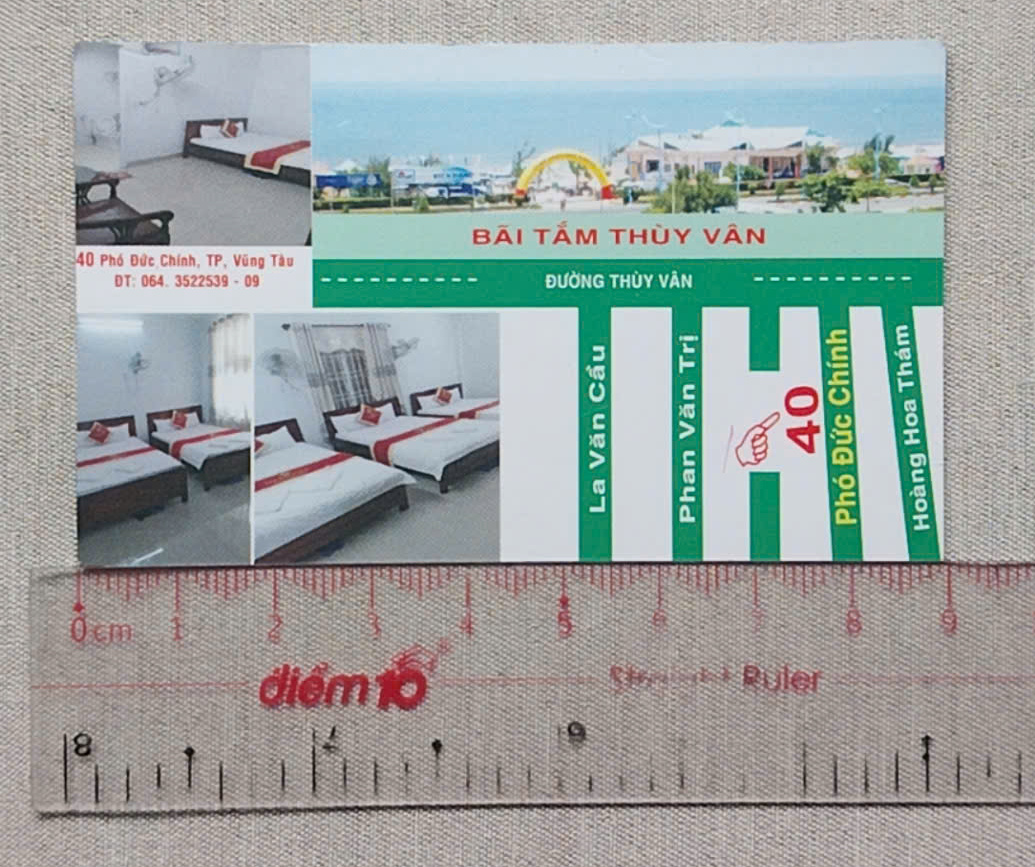
\includegraphics[width=0.5\textwidth]{pictures/section6/s6_p1_MeasuringObject.png}
                         \caption{Minh họa thiết lập hai camera song song}
                         \label{fig:stereo_setup}
                    \end{figure}
                    \item Chụp hai ảnh của vật thể từ hai camera song song, đảm bảo rằng vật thể nằm trong tầm nhìn của cả hai camera. Ở đây nhóm chọn 2 camera cách nhau 55 mm.
                    \begin{figure}[H]
                         \centering
                         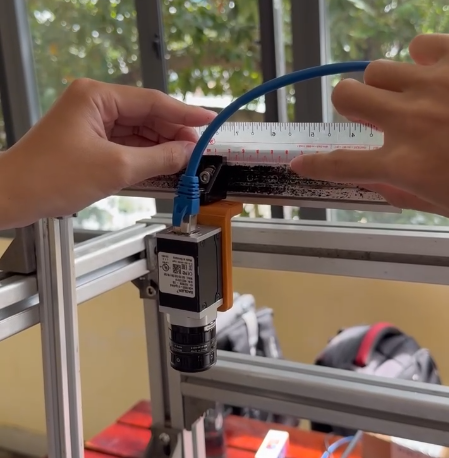
\includegraphics[width=0.5\textwidth]{pictures/section6/s6_p2_TakePhotoObject.png}
                         \caption{Ảnh chụp từ camera bên trái và bên phải}
                         \label{fig:stereo_images}
                    \end{figure}
               \end{itemize}
          \subsubsection{Buớc 2: Tính toán với Python}
               \begin{itemize}
                    \item Khai báo các biến cần thiết:
                    \begin{lstlisting}
script_dir = os.path.dirname(os.path.abspath(__file__))
calib_path = os.path.join(script_dir, "..", "Question_3", "camera_calibration.json")

LEFT_IMG_PATH  = os.path.join(script_dir, "images", "left.jpg")
RIGHT_IMG_PATH = os.path.join(script_dir, "images", "right.jpg")

pts_left = []
pts_right = []

B = 55  # Baseline in mm
                    \end{lstlisting} 
                    \item Tiến hành calibration hai camera sử dụng file JSON từ câu 3 và Undistort về cùng ma trận nội:
                    \begin{lstlisting}
with open(calib_path, 'r') as f:
     calib = json.load(f)
    
K_orig      = np.array(calib["camera_matrix"], dtype=np.float32)
dist_coeffs = np.array(calib["dist_coeffs"], dtype=np.float32)
K_new       = np.array(calib["new_camera_matrix"], dtype=np.float32)

imgL_raw = cv2.imread(LEFT_IMG_PATH)
imgR_raw = cv2.imread(RIGHT_IMG_PATH)
if imgL_raw is None or imgR_raw is None:
    raise SystemExit("Don't read LEFT/RIGHT images, check the path.")

h, w = imgL_raw.shape[:2]
Two pictures must have the same size!assert imgR_raw.shape[:2] == (h, w), ""

# Undistort to the same K_new
imgL = cv2.undistort(imgL_raw, K_orig, dist_coeffs, None, K_new)
imgR = cv2.undistort(imgR_raw, K_orig, dist_coeffs, None, K_new)
                    \end{lstlisting}
                    \item Chọn 2 điểm để đo khoảng cách trên hình và gọi event xử lý:
                    \begin{lstlisting}
def click_left(event, x, y, flags, param):
    if event == cv2.EVENT_LBUTTONDOWN and len(pts_left) < 2:
        pts_left.append((x, y))
        cv2.circle(param, (x, y), 3, (0, 255, 0), -1)
        if len(pts_left) == 1:
            _image = cv2.putText(param, 'P1', (x - 50, y - 50), cv2.FONT_HERSHEY_SIMPLEX,
                                 2, (255, 0, 0), 4, cv2.LINE_AA)
            cv2.imshow("Left image", _image)
            print(f"Left Point P1: ({x}, {y})")
        elif len(pts_left) == 2:
            cv2.line(param, pts_left[0], pts_left[1], (0, 255, 0), 2)
            _image = cv2.putText(param, 'P2', (x - 50, y - 50), cv2.FONT_HERSHEY_SIMPLEX,
                                2, (255, 0, 0), 4, cv2.LINE_AA)
            cv2.imshow("Left image", _image)
            print(f"Left Point P2: ({x}, {y})")
                    \end{lstlisting}
                    Xử lý tuơng tự với điểm bên phải.
                    \item Xem tâm tọa độ là camera bên trái, tính toán tọa độ 3D của điểm đã chọn từ các công thức trong Slide:
                    
                    \begin{lstlisting}
def point3d(u_left, v_left, u_right, v_right, K, B):
    f_x = K[0,0]
    f_y = K[1,1]
    cx = K[0, 2]
    cy = K[1, 2]
    d = u_left - u_right
    
    if abs(d) < 1e-6:
        raise ValueError("Can't compute depth.")

    Z = (f_x * B) / d 
    
    # X, Y (normalize to center)
    X = (u_left) * Z / f_x  
    Y = (v_left) * Z / f_y  
    return np.array([X, Y, Z]), d
                         \end{lstlisting}
               \end{itemize}
               
               